\newgeometry{top=2cm,left=2cm,right=2cm,bottom=2cm} 
%
\section{Classical properties of the BTZ spacetime}
As mentioned back in section 2.2, the BTZ spacetime has many features in common with black hole solutions in (3+1) dimensions, and in particular the Kerr black hole. As was pointed out during the derivation of the BTZ metric in section 2.2, a mass $M$ and angular momentum $J$ can be defined for the spacetime. It also posses two event horizons at:
%
%
\begin{equation}
r^2_{\pm}
=  \frac{\ell^2}{2} \, \left[
M \pm \sqrt{M^2 - \left(\frac{J}{\ell} \right)^2}
\right]
\end{equation}
As was also shown in section 2.2. Just like the Kerr black hole, the BTZ black hole also posses an \textbf{ergosphere}, which is a region between the outer horizon and the so-called \textbf{ergo shell}. In Schwarzschild-like coordinates, the ergo shell is defined as the hypersurafce on which $\partial_t$ becomes null, and thus:
%
%
\begin{equation}
g_{tt}(r) = 0
\quad \Rightarrow \quad
-M + \frac{r^2}{\ell^2} = 0
\quad \Rightarrow \quad
r_{erg}^2 = M \, \ell^2 \geq r_+^2
\end{equation}
%
%
The interesting thing about the ergosphere is that time-like curves in this region must partially be moving in the direction of $\partial_{\phi}$, as the only negative metric component in this region is $g_{t\phi}$.\newline
We have now exhausted the list of interesting properties of the BTZ spacetime which can easilly be extracted from its mettric. To better be able to investigate the causal properties of the BTZ spacetime, we now proceed to derive its conformal digram.

%%%%%%%%%%%%%%%%%%%%%%%%%%%%%%%%%%%%%
%\subsection{Mass and angular momentum}
%In order to properly define the mass and spin of the BTZ spactime, we will have to employ the \textbf{Chern-Simons formulation} of (2+1) dimensional gravity. As already discussed in section 2.3, the isometry group of $\widetilde{adS}$ is $SO(2,2)$. We first note that the Lie algebra $so(2,2)$ is isomorphic to the Lie algebra $iso(2,1)$; the Lie algebra of the (2+1) dimensional \textbf{Pioncaré group}. We can now use this fact to construct a $SO(2,2)$ 1-form potential usning the connection 1-forms ${\omega^i}_j$ and the triad frame $\epsilon^i$:
%%
%%
%\begin{equation}
%A := \frac{1}{2} \, \omega^{ij} \, \mathcal{J}_{ij} + \frac{1}{l} \, e^i \, \mathcal{P}_i
%\end{equation}
%%
%%
%Where $\mathcal{J}_{ij}$ and $\mathcal{P}_i$ are the rotation and translation generators of $iso(2,1)$ respectivly. It can now be shown that the \textbf{Einstein-Hilbert action} can be rewritten (\textit{up to boundary terms}) using a 3-form lagrangian $L(A)$ constructed from the potential $A$:
%%
%%
%\begin{equation}
%I_{EH}[A] = \frac{l}{2 \pi} \, \int_{\mathcal{M}} L(A)
%= \frac{l}{2 \pi} \, \int_{\mathcal{M}} \mathrm{Tr} \bigg[ A \wedge \mathrm{d}A + \frac{2}{3} \, A \wedge A \wedge A \bigg]
%\end{equation}
%%
%%
%Where $\mathrm{Tr}$ is defined such that $\mathrm{Tr}(\mathcal{J}_{ij} \, \mathcal{P}_k) = \varepsilon_{ijk}$, $\mathrm{Tr}(\mathcal{J}_{ij} \, \mathcal{J}_{kl}) = 0$ and $\mathrm{Tr}(\mathcal{P}_i \, \mathcal{P}_j) = 0$. It can now be shown that the variation of the lagrangian $L$ under the flow of a Killing vector $X$ is given by:
%%
%%
%\begin{equation}
%\mathcal{L}_X \, L = \mathrm{d}(i_X \, L) + i_x \, \mathrm{d}L = \mathrm{d}J = 0
%\quad , \quad
%J = i_X \, L = \frac{l}{2 \pi} \, \mathrm{d}\mathrm{Tr}(A \, i_X \, A)
%\end{equation}
%%
%%
%Where $i_X$ is the interior product (\textit{contraction operator}). We can now use the conserved current $J$ to define a conserved quantity corresponding to any given Killing vector $X$, by integrating over a spatial hyper-surface $\Sigma$:
%%
%%
%\begin{equation}
%Q[X] := \int_{\Sigma} J
%= \frac{l}{2 \pi} \, \int_{\partial \Sigma} \mathrm{d}\mathrm{Tr}(A \, i_X \, A)
%= \frac{1}{2 \pi} \, \int_{\partial \Sigma} \frac{1}{2} \varepsilon_{ijk} \, \big(
%\omega^{ij} \, \epsilon^k(X)
%+ \omega^{ij}(X) \, \epsilon^k
%\big)
%\end{equation}
%%
%%
%We can now define the mass and angular momentum of the BTZ spacetime using its two Killing vectors $\partial_t$ and $\partial_{\phi}$. In section 2.2, we defined a triad for the BTZ metric and found the corresponding connection 1-forms, and using those expressions we find that:
%%
%%
%\begin{equation}
%\frac{1}{2} \varepsilon_{ijk} \, \big(
%\omega^{ij} \, \epsilon^k(\partial_t)
%+ \omega^{ij}(\partial_t) \, \epsilon^k
%\big)
%= M \, \mathrm{d}\phi + \frac{J}{l^2} \, \mathrm{d}t
%\end{equation}
%%
%%
%\begin{equation}
%\frac{1}{2} \varepsilon_{ijk} \, \big(
%\omega^{ij} \, \epsilon^k(\partial_{\phi})
%+ \omega^{ij}(\partial_{\phi}) \, \epsilon^k
%\big)
%= J \, \mathrm{d}\phi + M \, \mathrm{d}t
%\end{equation}
%%
%%
%Thus, if we choose $\Sigma$ to be a surface of constant $t$, we can integrate the above expressions to find:
%%
%%
%\begin{equation}
%Q[\partial_t] = M
%\quad , \quad
%Q[\partial_{\phi}] = J
%\end{equation}
%%%%%%%%%%%%%%%%%%%%%%%%%%%%%%%%%%%%%

\subsection{Causal structure of the spacetime}
We will here focus on deriving a conformal digram for the case of $J=0$; the static BTZ black hole. The metric for the static BTZ black hole is given by:
%
%
\begin{equation}\label{static_btz}
ds^2 = -f^2(r) \, \mathrm{d}t^2
+ f^{-2}(r) \, \mathrm{d}r^2
+ r^2 \mathrm{d}\phi^2
\quad , \quad
f^2(r) = -M + \frac{r^2}{\ell^2}
\end{equation}
%
\begin{equation*}
-\infty < t < \infty \, , \quad 0 < r < \infty \, , \quad 0 \leq \phi < 2 \pi
\end{equation*}
%
%
Because this metric is so similar to the (3+1)-dimensional Schwarzschild black hole, we can follow the usual derivation as seen in \cite{GR} of Kruskal coordinates and a Penrose diagram quite closely.\newline
%
%
%
Before we start, we note that just like in the Schwarzschild metric, there appears to be a singularity at $r = r_+ = \ell \, \sqrt{M}$. As was the case with Schwarzschild, this is merely a coordinate singularity. Because it is shown in the exact same way as for Schwarzschild, we will not go through any trouble showing it explicitly, but it will be apparent once we see the conformal diagram.
We start by introducing a so-called turtoise coordinate $r^*$, such that:
%
%
\begin{equation}
f^2(r) \, (\mathrm{d}r^*)^2
= f^{-2}(r) \, \mathrm{d}r^2
\quad \Rightarrow \quad
\frac{\mathrm{d}r^*}{\mathrm{d}r} = f^{-2}(r)
\end{equation}
%
%
\begin{equation}
\Rightarrow \quad
r^*(r) = \int \frac{1}{\frac{r^2}{\ell^2} - M} dr =
\frac{\ell^2}{2 r_+} \int \frac{1}{r - r_+} - \frac{1}{r + r_+} dr =
\frac{\ell^2}{2 r_+} \ln \left( \frac{|r - r_+|}{r + r_+} \right)
\end{equation}
%
%
We see that the $r^*(r)$ is singular at $r = r_+$, so we only look at the case $r > r_+$, for which we do not need the absolute value.
%
%
%
By changing to the turtoise coordinate, we can bring the metric to the form:
%
%
\begin{equation}
ds^2 = f^2(r) \, \left[- \mathrm{d}t^2 + (\mathrm{d}r^*)^2 \right] + r^2(r^*) \, \mathrm{d}\phi^2
\end{equation}
\begin{equation*}
-\infty < t < \infty
\quad , \quad
-\infty < r^* < 0
\end{equation*}
%
%
%
It it is now straightforward to define a pair of null coordinates $v$ and $u$, using the above metric:
%
%
\begin{equation}
v = t + r^*
\qquad,\qquad
u = t - r^*
\end{equation}
%
%
In terms of the new null coordinates $v$ and $u$, the static BTZ metric now takes the following form:
%
%
\begin{equation}
ds^2 = - \frac{f^2(r)}{2} \, \left[ \mathrm{d}u \, \mathrm{d}v
+ \mathrm{d}v \, \mathrm{d}u \right]
+ r^2 \, \mathrm{d}\phi^2
\end{equation}
%
\begin{equation*}
-\infty < u, v < \infty 
\quad , \quad
v < u
\end{equation*}
%
%
We note that $r$ is now to be interpreted as an implicit function of $v$ and $u$, with the following relation:
%
%
\begin{equation}
\frac{1}{2}(v - u)
= \frac{\ell^2}{2 r_+} \ln \left( \frac{r - r_+}{r + r_+} \right)
\end{equation}
%
%
%
Just like in the Schwarzschild case, the apparent coordinate singularity at $r = r_+$ is moved to infinity in these coordinates. Fixing it requires us to write $u$ and $v$ in terms of our initial coordinates $t$ and $r$:
%
%
\begin{equation}
v = t + r^*
= t + \frac{\ell^2}{2 r_+} \ln \left( \frac{r - r_+}{r + r_+} \right)
\qquad , \qquad 
u = t - r^*
= t - \frac{\ell^2}{2 r_+} \ln \left( \frac{r - r_+}{r + r_+} \right)
\end{equation}
%
%
%
We see now that a clever choice of coordinates $v'$ and $u'$, might be given by the following:
%
%
\begin{equation}
v' = \exp \left( \frac{r_+ v}{\ell^2}\right) \qquad , \qquad
u' = - \exp \left( \frac{-r_+ u}{\ell^2}\right)
\end{equation}
%
%
These can be expressed in terms of the original coordinates $t$ and $r$, in the following way:
%
%
\begin{equation}
v' = \sqrt{\frac{r - r_+}{r + r_+}} \exp \left( \frac{r_+ t}{\ell^2}\right) \qquad , \qquad
u' = -\sqrt{\frac{r - r_+}{r + r_+}} \exp \left( \frac{- r_+ t}{\ell^2}\right)
\end{equation}
%
%
In terms of the coordinates $v'$ and $u'$, the static BTZ metric now takes the following form:
%
%
\begin{equation}
ds^2 = - \frac{f^2(r)}{2} \, \frac{\ell^4}{r_+^2} \,
\left( \frac{r + r_+}{r - r_+} \right) \left[ \mathrm{d}u' \mathrm{d}v' + \mathrm{d}v' \mathrm{d}u'\right]
+ r^2 \, \mathrm{d}\phi^2
\end{equation}
%
\begin{equation*}
0 < v' < \infty
\quad , \quad
-\infty < u' < 0
\quad , \quad
v' \, u' < -1
\end{equation*}
%
%
%
We can simplify the above metric a bit by realizing that:
%
%
\begin{equation}\label{fsimply}
f^2(r) = -M + \frac{r^2}{\ell^2}
= \frac{r^2 - r_+^2}{l^2}
= \frac{(r - r_+)(r + r_+)}{\ell^2}
= \frac{(r + r_+)^2}{\ell^2} \left( \frac{r - r_+}{r + r_+} \right)
\end{equation}
%
%
Using the above expression for $f^2(r)$, we now find that:
%
%
\begin{equation} \label{premetric}
ds^2 = - \frac{\ell^2}{2} \, \frac{(r + r_+)^2}{r_+^2} \, \left[ \mathrm{d}u' \mathrm{d}v' + \mathrm{d}v' \mathrm{d}u' \right]
+ r^2 \mathrm{d}\phi^2
\end{equation}
%
%\begin{equation*}
%0 < v' < \infty
%\quad , \quad
%-\infty < u' < 0
%\quad , \quad
%0 \leq \phi < 2 \pi
%\end{equation*}
%
%
%
It is now apparent that $r = r_+$ is not a real singularity, since the metric is not singular for this value of $r$ in these coordinates. To get the Kruskal.like coordinates for the BTZ black holes, we just need to change back into a set of one time-like and two space-like coordinates, using the combination:
%
%
\begin{equation}\label{RandT}
T = \frac{1}{2} \, (v' + u') \qquad , \qquad
R = \frac{1}{2} \, (v' - u')
\end{equation}
%
%
We can now write the coordinates $T$ and $R$, in terms of the original coordinates $t$ and $r$:
%
%
\begin{equation}\label{RightT}
T = \frac{1}{2} \, \sqrt{\frac{r - r_+}{r + r_+}} \, \left[
\exp \left( \frac{r_+ t}{\ell^2}\right)
-
\exp \left( \frac{- r_+ t}{\ell^2}\right)
\right] 
= \sqrt{\frac{r - r_+}{r + r_+}} \, \sinh \left( \frac{r_+ t}{\ell^2}\right)
\end{equation}
%
%
\begin{equation}\label{RightR}
R = \frac{1}{2} \, \sqrt{\frac{r - r_+}{r + r_+}} \, \left[
\exp \left( \frac{r_+ t}{\ell^2}\right)
+
\exp \left( \frac{- r_+ t}{\ell^2}\right)
\right] 
= \sqrt{\frac{r - r_+}{r + r_+}} \, \cosh \left( \frac{r_+ t}{\ell^2}\right)
\end{equation}
%
%
The metric for the static BTZ balck hole, now takes a particularly simple form, in terms of $T$ and $R$:
%
%
\begin{equation}
ds^2 = \ell^2 \, \frac{(r + r_+)^2}{r_+^2} \, \left[
-\mathrm{d}T^2
+ \mathrm{d}R^2 \right]
+ r^2 \, \mathrm{d}\phi^2
\end{equation}
%
\begin{equation*}
-\infty < T, R < \infty
\quad , \quad
-1 < R^2 - T^2 < 1
\quad , \quad
0 \leq \phi < 2 \pi
\end{equation*}
%
%
%
It is easily seen from (\ref{RightR}) and (\ref{RandT}), that $R^2 - T^2 > 0$ and $R > 0$, for $r > r_+$. But space-like geodesics can reach $R = 0$ at finite parameter value, so there must be more spacetime beyond this. We can cover this other patch by a set of coordinates similar to (\ref{RightR}) and (\ref{RightT}), but with a minus sign on each coordinate (\textit{so that $R < 0$; we see that these two patches do not overlap}). \newline
When we defined the turtoise coordinate $r^*$, we noted that it was singular at $r = r_+$, and chose to look at only $r > r_+$. Had we instead chosen $0 < r < r_+$, we would have simply swapped the order of $r_+$ and $r$ when we removed the absolute value, such that:
%
%
\begin{equation}
r^* = \frac{\ell^2}{2 r_+} \ln \left( \frac{r_+ - r}{r + r_+} \right)
\end{equation}
%
%
This would have given us a minus sign in (\ref{fsimply}), which would have lead to us swapping the definitions of $T$ and $R$ in (\ref{RandT}), and consequently the definitions of $T$ and $R$ in terms of $t$ and $r$ would be swapped as well. This would correspond to a patch in which $R^2 - T^2 < 0$ and $T > 0$. In this patch of spacetime, it is possible for time-like geodesics to reach $T = 0$ at finite parameter value, so there must be more spacetime beyond this as well. We can, once again, cover this new patch by simply adding a minus sign to each coordinate $T$ and $R$. This leaves us with the maximally extended spacetime for the static BTZ black hole, consisting of four patches with the following coordinates:\newline
\newline
%
%
\noindent
\textbf{I} \qquad ($r_+ < r$)
%
\begin{equation}
T = \sqrt{\frac{r - r_+}{r + r_+}} \sinh \left( \frac{r_+ t}{\ell^2}\right)
\qquad , \qquad
R = \sqrt{\frac{r - r_+}{r + r_+}} \cosh \left( \frac{r_+ t}{\ell^2}\right)
\end{equation}
%
%
\textbf{II} \qquad ($0 < r < r_+$)
%
\begin{equation}
T = \sqrt{\frac{r_+ - r}{r + r_+}} \cosh \left( \frac{r_+ t}{\ell^2}\right)
\qquad , \qquad
R = \sqrt{\frac{r_+ - r}{r + r_+}} \sinh \left( \frac{r_+ t}{\ell^2}\right)
\end{equation}
%
%
\textbf{III} \qquad ($r_+ < r$)
%
\begin{equation}
T = - \sqrt{\frac{r - r_+}{r + r_+}} \sinh \left( \frac{r_+ t}{\ell^2}\right)
\qquad , \qquad
R = - \sqrt{\frac{r - r_+}{r + r_+}} \cosh \left( \frac{r_+ t}{\ell^2}\right)
\end{equation}
%
%
\textbf{IV} \qquad ($0 < r < r_+$)
%
\begin{equation}
T = - \sqrt{\frac{r_+ - r}{r + r_+}} \cosh \left( \frac{r_+ t}{\ell^2}\right)
\qquad , \qquad
R = - \sqrt{\frac{r_+ - r}{r + r_+}} \sinh \left( \frac{r_+ t}{\ell^2}\right)
\end{equation}\newline
%
%
\begin{figure}[h!]
%
\centering
%
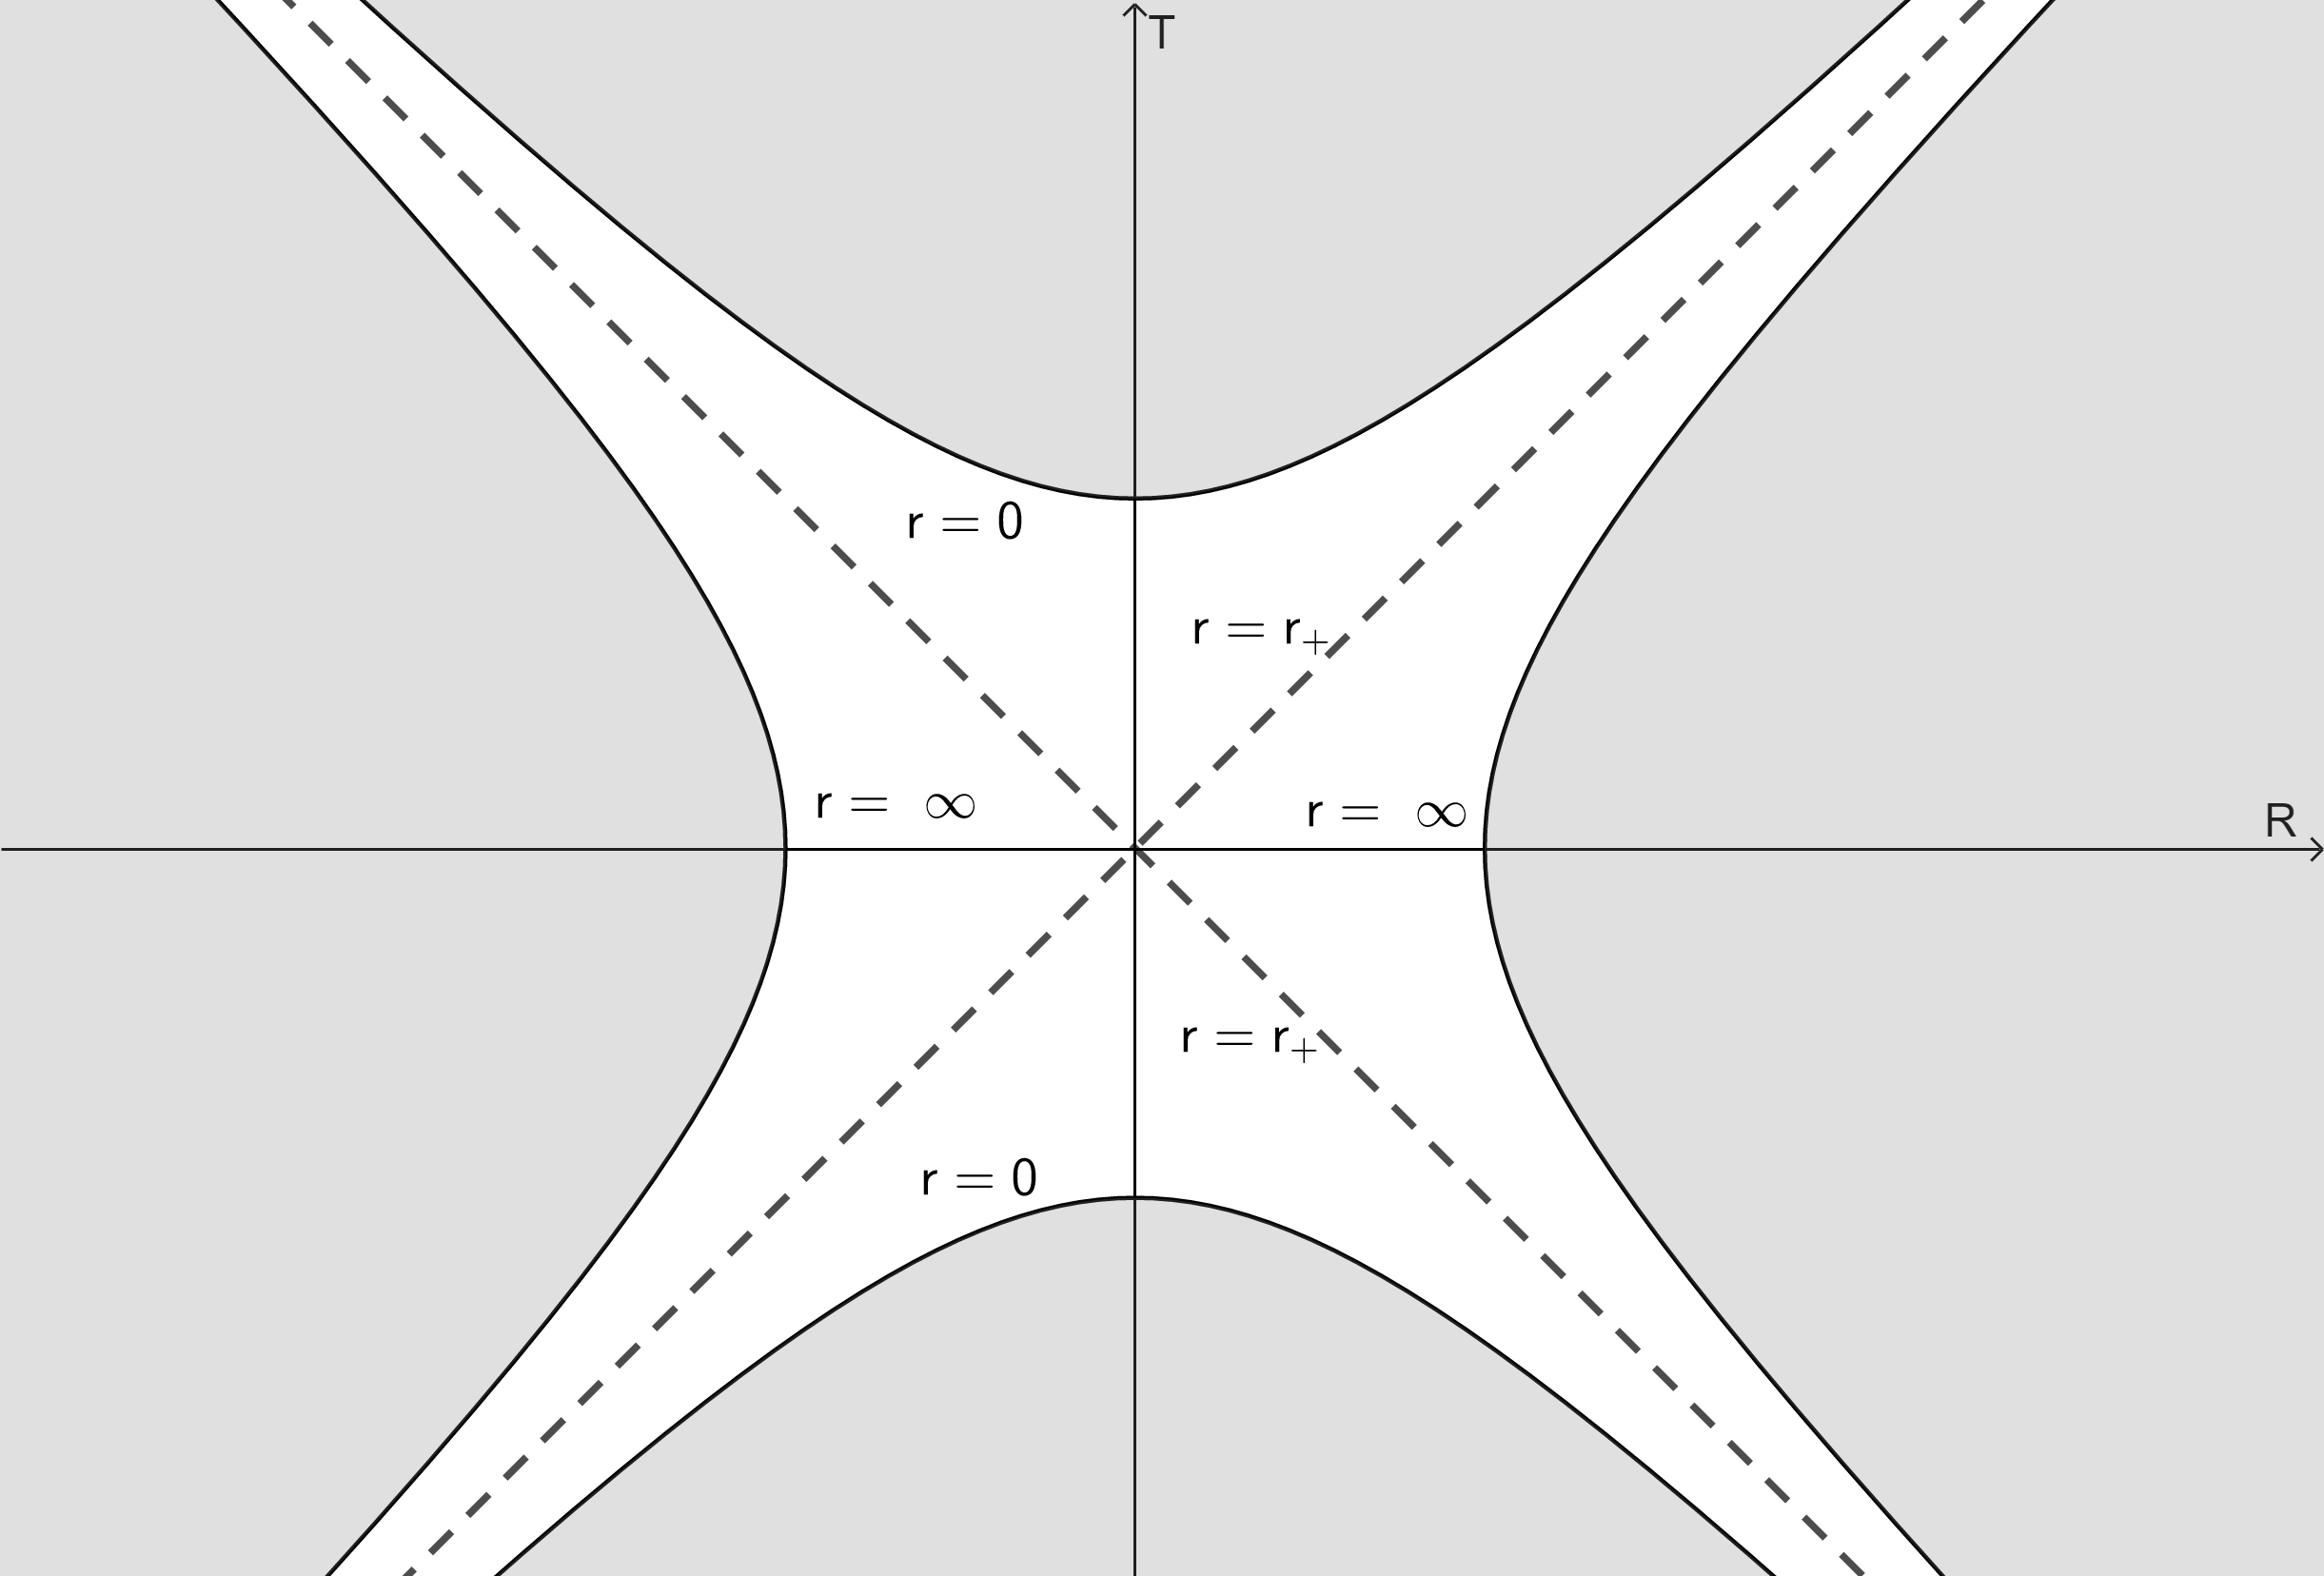
\includegraphics[width=0.80\textwidth]{../pics/Kruskal_static.png}
%
\caption{The Kruskal-diagram for the static BTZ black hole. Light rays move on $45^{\circ}$ lines in these coordinates. The past and future event horizons are null surfaces located at $r=r_+$. The grey areas are not part of the spacetime.}
%
\label{fig:kruskal_static}
%
\end{figure}\newline \noindent
%
%
Patch I and III corresponds to two different asymptotically $AdS_3$ parts of the spacetime (\textit{as will be clear when the conformal digram is constructed}), while II and IV are the black and white hole respectively. In patch I and III, we see that $r = const$ corresponds to $0 < R^2 - T^2 = const < 1$, while $t = const$ corresponds to $-1 < T / R = const < 1$. This means that constant $r$ curves are hyperbolas while constant $t$ curves are lines intersecting the origin, just as in the Schwarzschild case. The point at $r = 0$ lies in patch II and IV, and are described by the hyperbolas:
%
%
%\begin{equation}
%T_0 = \cosh \left( \frac{r_+ t}{\ell^2} \right) \qquad , \qquad
%R_0 = \sinh \left( \frac{r_+ t}{\ell^2} \right)
%\end{equation}
\begin{equation}
R^2 - T^2 = -1
\end{equation}
%
%
%
Which is again just like the Schwarzschild case. Different from the Schwarzschild case however, is $r = \infty$, which usually lies at $R^2 - T^2 = \infty$, but now lies in patch I and III, and are described by:
%
%
%\begin{equation}
%T_\infty = \sinh \left( \frac{r_+ t}{\ell^2} \right) \qquad , \qquad
%R_\infty = \cosh \left( \frac{r_+ t}{\ell^2} \right)
%\end{equation}
\begin{equation}
R^2 - T^2 = 1
\end{equation}
%
%
%
If we want to construct a conformal diagram for the static BTZ spacetime, we can follow the approach of not only Schwarschild but also flat space, and make another coordinate transformation:
%
%
\begin{equation}
v' = \tan \left( r_+ V \right)
\qquad , \qquad
u' = \tan \left( r_+ U \right)
\end{equation}
%
%
\begin{equation}
\Rightarrow \quad
\mathrm{d} v' = \frac{r_+}{\cos^2(r_+ V)} \mathrm{d}V
\qquad , \qquad
\mathrm{d} u' = \frac{r_+}{\cos^2(r_+ U)} \mathrm{d}U
\end{equation}
%
%
\begin{equation}
\Rightarrow \quad
\mathrm{d} v' \mathrm{d} u' + \mathrm{d} u' \mathrm{d} v' =
\frac{{r_+}^2}{\cos^2(\frac{V}{r_+}) \cos^2(\frac{U}{r_+})} \left[ \mathrm{d}V \mathrm{d}U + \mathrm{d}U \mathrm{d}V \right]
\end{equation}
%
%
We can now write the metric (\ref{premetric}), using the coordinates $V$ and $U$, in the follow way:
%
%
\begin{equation}
ds^2 = - \frac{\ell^2}{2} \, \frac{(r + r_+)^2}{\cos^2(r_+ V) \cos^2(r_+ U)} \left[ \mathrm{d}V \mathrm{d}U + \mathrm{d}U \mathrm{d}V \right]
+ r^2  \, \mathrm{d}\phi^2
\end{equation}
%
\begin{equation*}
0 < V < \pi/2
\quad , \quad
-\pi/2 < U < 0
\quad , \quad
0 \leq \phi < 2 \pi
\end{equation*}
%
%
We now make one last transformation to one time-like and one space-like coordinate, $T'$ and $R'$:
%
%
\begin{equation}
V = \frac{1}{2} \, (T' + R')
\qquad , \qquad
U = \frac{1}{2} \, (T' - R')
\end{equation}
%
%
In terms of the time-like coordinate $T'$ and space-like coordinate $R'$, the metric finally takes the form:
%
% This equation should not have two numbers (fixed)
%
\begin{align}
ds^2 & = \omega^{-2} \, \left[- (\mathrm{d}T')^2 + (\mathrm{d}R')^2 \right]
+ r^2 \, \mathrm{d}\phi^2
\notag\\
\omega^{-2} & = \frac{2 \, \ell^2 \, (r + r_+)^2}{\left[ \cos(r_+ T') + \cos(r_+ R') \right]^2}
\end{align}
%
\begin{equation*}
-\pi/2 < T', R' < \pi/2
\quad , \quad
0 \leq \phi < 2 \pi
\end{equation*}
%
%
If we omit the angular part of the above metric, we now easily see that the rest of the metric is related by the conformal factor $\omega^2$ to the metric of flat two dimensional Minkowski space:
%
%
\begin{equation}
\tilde{ds}^2 = - (\mathrm{d}T')^2 + (\mathrm{d}R')^2
\end{equation}
\begin{equation*}
-\pi/2 < T', R' < \pi/2
\end{equation*}
%
%
Having found these coordinates, we can now draw the conformal diagram for the static BTZ Black Hole. It will look like the Schwarzschild Black Hole near the event horizon, but will have the same structure at conformal infinity as $AdS_3$:
%
%
\begin{figure}[h!]
%
\centering
%
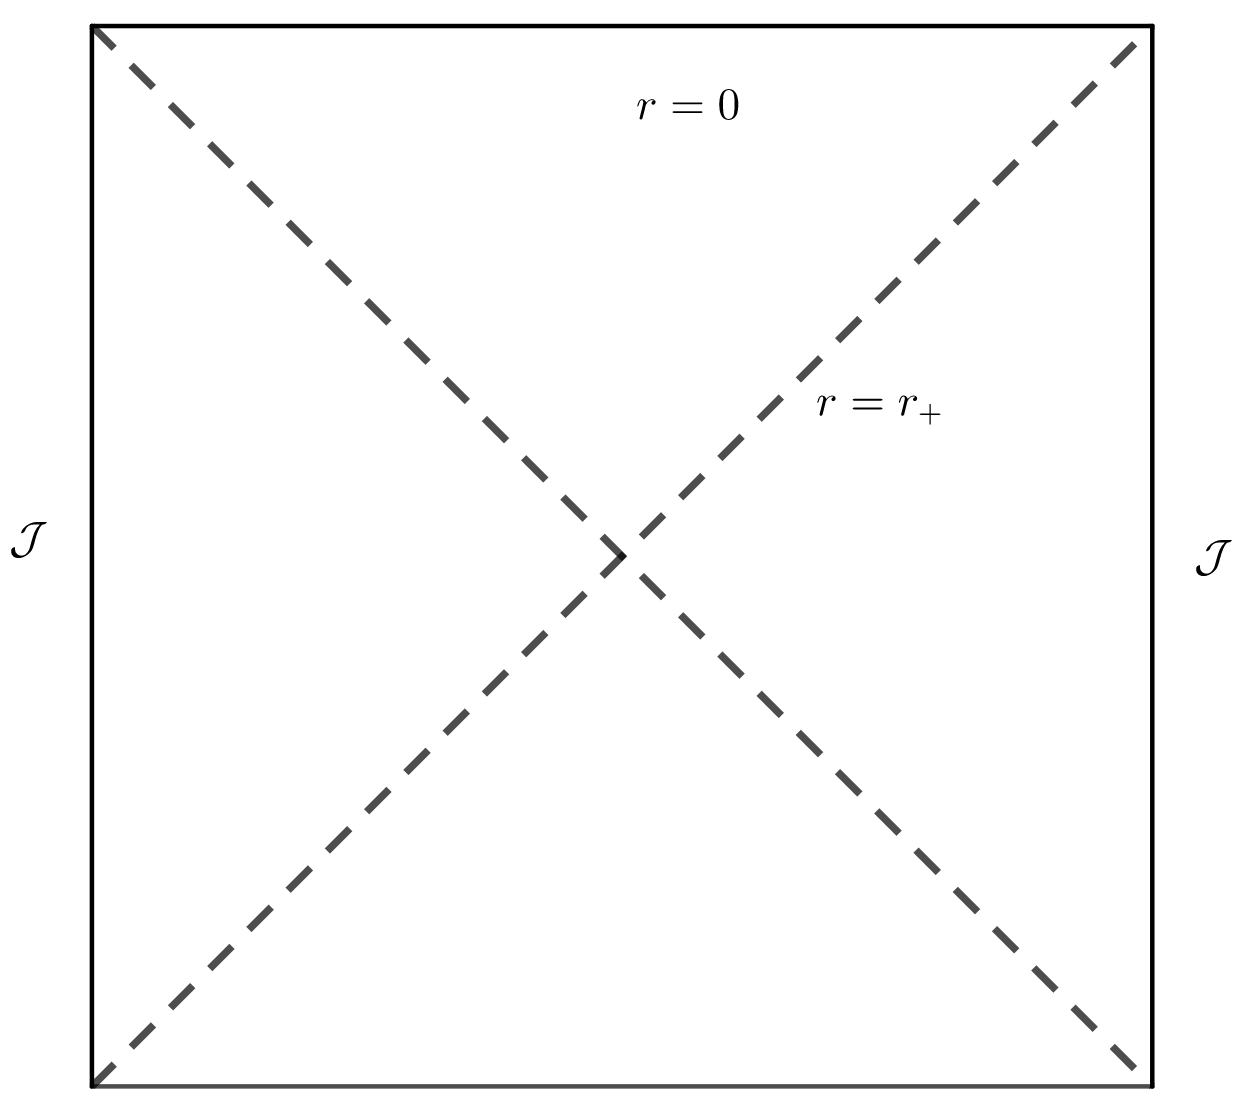
\includegraphics[width=0.6\textwidth]{../pics/BTZ_stat_Pen.png}
%
\caption{The conformal diagram for the static BTZ black hole. The past and future event horizons are again located at $r=r_+$. In this digram, we now see that the spacetime is asymptotically $AdS_3$.}
%
\label{fig:pen_btz_static}
%
\end{figure}
%
%
%%%%%%%%%%%%%%%%%%%%%%%%%%%%%%%%%%%%%
%\begin{figure}[h!]
%%
%\centering
%%
%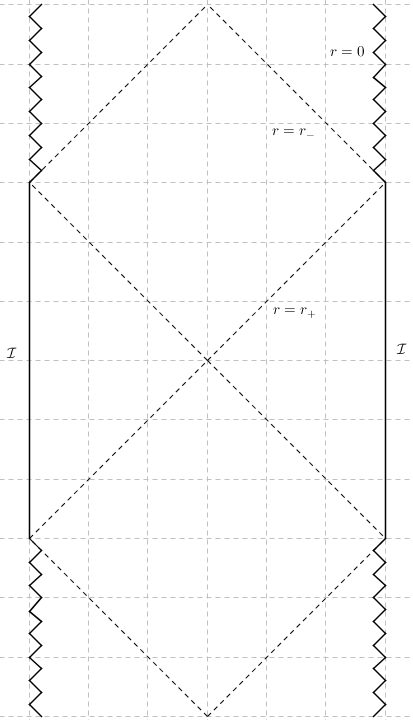
\includegraphics[width=0.6\textwidth]{../pics/BTZ.png}
%%
%\caption{The conformal diagram for the rotating BTZ black hole. In this digram, we can now easily see that the spacetime is asymptotically $AdS_3$.}
%%
%\label{fig:pen_btz}
%%
%\end{figure}
%%%%%%%%%%%%%%%%%%%%%%%%%%%%%%%%%%%%%

\newpage

\subsection{Singularities}
As we have already seen in the previous subsection, the apparent singularities at the inner and outer horizon are coordinate dependent singularities, as is also the case for black hole solutions in (3+1) dimensions. Therefore, one would expect the curvature to stay finite on the horizons. In order to check this, and to identify any other potential curvature singularites of the BTZ black hole, we can compute the \textbf{curvature invariant} $R_{ijkl} \, R^{ijkl}$. Using the expression we obtained in section 1.3, for the Riemann tensor associated with vacuum solutions to Einsteins Equations, we find that:
%
%
\begin{equation}
R_{ijkl} \, R^{ijkl}
= \Lambda^2 \, (g_{\rho\mu} \, g_{\nu\sigma} - g_{\rho\nu} \, g_{\mu\sigma}) \, 
(g^{\rho\mu} \, g^{\nu\sigma} - g^{\rho\nu} \, g^{\mu\sigma})
= 12 \, \Lambda^2
\end{equation}
%
%
It is now evident, that the BTZ black hole has no curvature singularities anywhere. This is very different from black holes in (3+1) dimensions, which all possess some kind of curvature singularity in their interior. Although the BTZ black hole possess no curvature singularities, another complication arise if we try to extend the spacetime to $r^2<0$; the emergence of \textbf{closed time-like curves}. This is most easily seen by performing the following change of coordinate:
%
%
\begin{equation}
\tilde{r} = r^2
\quad \Rightarrow \quad
\mathrm{d}\tilde{r} = 2 \, r \, \mathrm{d}r
\quad \Rightarrow \quad
\mathrm{d}r^2 = \frac{1}{4 \, \tilde{r}} \, \mathrm{d}\tilde{r}^2
\end{equation}
%
%
With this change of coordinate, the static BTZ metric now takes on the following form:
\begin{equation}
ds^2 = -\bigg[-M + \frac{\tilde{r}}{l^2} \bigg] \, \mathrm{d}t^2
+ \frac{1}{4 \, \tilde{r}} \, \bigg[-M + \frac{\tilde{r}}{l^2} \bigg]^{-1} \, \mathrm{d}\tilde{r}^2
+ \tilde{r} \, \mathrm{d}\phi^2
\end{equation}
%
%
If we now extend the range of $\tilde{r}$ such that $\tilde{r} \in (-\infty, \infty)$, it is now clear that for example curves of constant $t$ and $\tilde{r}$ become time-like for $\tilde{r} < 0$. Because $\phi$ is compact with $\phi \sim \phi + 2 \pi$, these curves can always be chosen to be closed. Because of the existence of closed time-like curves in the region $\tilde{r} < 0$, this part of the spacetime is usually excluded from the rest of the BTZ spacetime, and $\tilde{r} = 0$ is called a \textbf{causal singularity} of the spacetime. This rather exotic causal singularity at $\tilde{r} = 0$ will in fact become a \textbf{conical singularity} whenever the event horizon at $r^2_+$ lies in the region of negative $\tilde{r}$. Because $r^2_+ = \ell^2 \, M$, this happens when $M < 0$. To see this, we now perform the following change of coordinate:
%
%
\begin{equation}
\rho = \frac{1}{\mu^2} \, \sinh^{-1} \left( \frac{r}{\mu \, \ell} \right)
\quad , \quad
\mu^2 := -M
\end{equation}
%
%
We can now express $r^2$ and $f^2(r)$ in terms of the new radial coordinate $\rho$:
%
%
\begin{equation}
f^2(r) = \mu^2 + \frac{r^2}{\ell^2}
= \mu^2 \, \cosh^2(\rho \, \mu^2)
\quad , \quad
r^2 = \ell^2 \, \mu^2 \, \sinh^2(\rho \, \mu^2)
\end{equation}
%
%
In terms of $\rho$, the static BTZ metric (\ref{static_btz}), now takes the following form:
%
%
\begin{equation}
ds^2 = -\mu^2 \, \cosh^2(\rho \, \mu^2) \, \mathrm{d}t^2
+ \mathrm{d}\rho^2
+ \ell^2 \, \mu^2 \, \sinh^2(\rho \, \mu^2) \, \mathrm{d}\phi^2
\end{equation}
%
%
Close to $r=0 \Leftrightarrow \rho = 0$, the metric now takes the following approximate form to leading order in $\rho$:
%
%
\begin{equation}
ds^2 \approx -\mu^2 \, \mathrm{d}t^2
+ \mathrm{d}\rho^2
+ \ell^2 \, \rho^2 \, \mathrm{d}\tilde{\phi}^2
\quad , \quad
\tilde{\phi} \in (0, 2 \pi \mu^2)
\end{equation}
%
%
It is now manifestly clear, that the static BTZ spactime for $M < 0$ has a conical singularity in the $(\rho, \phi)$-plane, at $\rho = 0$, with a deficit angle of $\alpha = 1-\mu^2$. As mentioned ealier, the event horizon at $r^2_+ = \ell^2 \, M$ lies beyond the conical singularity at $r=0$, and it is thus a \textbf{naked singularity}. As discussed in \cite{2+1 black hole}, these same phenomena happen for the general BTZ spacetime when $J^2 > \ell^2 \, M^2$.
